\documentclass[a4paper,12pt]{scrreprt}
\usepackage[T1]{fontenc}
\usepackage[utf8]{inputenc}
\usepackage[ngerman]{babel}
\usepackage[table]{xcolor}
% http://ctan.org/pkg/xcolor
\usepackage{tabu}
\usepackage{graphicx}
\usepackage{lmodern}
\usepackage{hyperref}
\usepackage{geometry}
\geometry{verbose,a4paper,tmargin=20mm,bmargin=20mm,lmargin=30mm,rmargin=30mm}



\begin{document}


%\titlehead{Kopf} %Optionale Kopfzeile
\author{Alexander Rieppel} %Zwei Autoren
\title{Transportlogistik} %Titel/Thema
\subject{Betriebs- und Informationsmanagement} %Fach
\subtitle{Ausarbeitung} %Genaueres Thema, Optional
\date{\today} %Datum
\publishers{5AHITT} %Klasse
{\Huge }

\maketitle
\tableofcontents


\chapter{Einführung}
	Der Begriff Transportlogistik beschreibt die Lieferung und Beförderung von Gütern, zwischen verschiedenen Orten innerhalb von Transportnetzwerken. Dieser Teilbereich der Logistik ist durch den heutigen Wohlstand entstanden, in dem sich Unternehmen auf ihre Kernkompetenzen konzentrieren und darüber hinausgehende Dienstleistungen und Produkte europaweit und international einkaufen. Die Planung und Optimierung, Ausführung, Überwachung und Steuerung der damit verbundenen Güterströme ist Aufgabe der Transportlogistik. Neben dem Transport von Waren als solches wird auch die Be- und Entladung zur Transportlogistik gezählt.\\
	
	Das Problem Güter von A nach B zu bringen ist für jeden Unternehmer eine Herausforderung. Prinzipiell ist es dabei egal, ob die Ware per LKW, Zug, Schiff, Flugzeug, Pipeline, etc. transportiert wird. Es geht rein darum, dass die Ware ankommt, sie möglichst unbeschadet ankommt und vor allem schnell am Ziel ist. Auch der Kostenfaktor spielt dabei eine große Rolle und auch ökologische Nachhaltigkeit gewinnt zunehmend an Bedeutung.\\
	
	Obwohl es im Prinzip egal ist womit transportiert wird, ist der am meisten genutzte Verkehrsträger zur Güterbeförderung, speziell hierzulande, die Straße. Zu den entscheidenden Gründen zählt die Netzbildungsfähigkeit des LKW, der jede Quelle und Senke flexibel erreichen kann. Die Stärke von Schiene und Binnenwasser-straße liegen in dem effizienten Transport von Massengütern über längere Strecken. Für die besonders langen Distanzen im internationalen Gütertransport werden das Seeschiff für große Volumina und das Flugzeug eher für besonders eilige oder wertvolle Fracht genutzt. Neben der reinen Beförderung als offensichtlichste transportlogistische Funktion erfordern die Ver- und Entsorgung von Industrie- und Handelsunternehmen weitere Leistungen, wie die Lagerhaltung für die zeitliche Überbrückung zwischen Fertigung und Absatz, den Umschlag im Rahmen des Verkehrsmittelwechsels und die Kommissionierung zur Vereinzelung nachgefragter Mengen. Hinzu kommen verstärkt auch Tätigkeiten, die einen zusätzlichen Mehrwert am Gut schaffen, wie die Montage von Teilen zu Modulen, die Aufarbeitung von Produkten, ihre Etikettierung oder Sequenzierung.\\
	
	Dies zeigt auch, dass die Gütertransportlogistik steigenden
	Anforderungen unterliegt, durch einen stetigen Anstieg gekennzeichnet ist, aber auch eine Fülle von Gestaltungsmöglichkeiten bietet. Dies belegt die Bedeutung der Transportlogistik mit der Folge, dass sich Gesellschaft, Wirtschaft und Wissenschaft intensiv mit Fragestellungen auf diesem Gebiet auseinander setzen müssen.\\\\
	Zu den Zielen der Transportlogistik gehören:
	\begin{itemize}
	\item Effektivität - die Aufgaben werden erfüllt
	\item Effizienz - die Aufgaben werden mit einem günstigen Kosten-Nutzen Verhältnis erfüllt
	\item Sicherheit - Gegen technische Störungen, Unfälle, etc. wird vorgebeugt
	\item Robustheit - Transportketten arbeiten auch im Fall von Störungen und Auftragsschwankungen zuverlässig
	\item Nachhaltigkeit - Neben ökonomischen Belangen sind ökologische und soziale Interessen zu berücksichtigen
	\item Wirtschaftlichkeit - Die Kosten sind angemessen und die erzielbaren Erträge decken für alle beteiligten die Aufwände
	\end{itemize}
	
	\begin{figure}
\centering
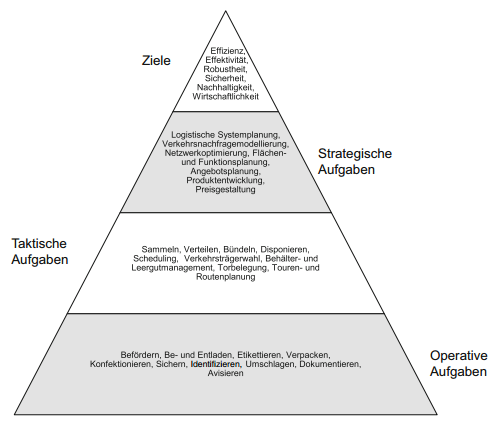
\includegraphics[width=1\linewidth]{./Ziele_Transportlogistik}
\caption{Ziele der Transportlogistik und Aufgaben}
\label{fig:Ziele_Transportlogistik}
\end{figure}

	\chapter{Wirtschaftliche Aspekte der Transportlogistik}
	
	Die Logistik ist für sämtliche Industriebranchen ein maßgeblicher Faktor. Insbesondere sind die Chemiebranche, die Stahlbranche, die Automobilbranche und das verarbeitende Gewerbe, von einem reibungslosen Ablauf der Logistik abhängig, um ihre Wertschöpfungskette aufrecht erhalten zu können. Die erforderlichen Transporte erstrecken sich über die ganze Welt. Sie finden zwischen verschiedenen Partnern der Wertschöpfungskette, von der Rohstoffgewinnung, über die Verarbeitung und den Handel bis hin zum Endkunden statt. Die Partner innerhalb der Wertschöpfungskette können verschiedenen Industrien angehören. Beispielsweise ist die Stahl- und Metallindustrie ein wesentlicher Zulieferer der Automobilindustrie.\\
	
	Die Transportlogistik nimmt im Vergleich international eine Schlüsselposition ein. Mit einem weltweiten Marktvolumen von 4.200 Mrd. Euro ist die Logistik nach der Automobilindustrie und dem Maschinenbau die drittgrößte Branche. Alleine in Europa erzielte die Logistik 2009 ein Martvolumen von 880 Mrd. Euro. Von diesen erbrachten Logistikleistungen entfallen - gemessen in Wertschöpfung - mehr als ein Drittel auf das Transportgeschäft. Damit ist die Transportlogistik eine wichtige Branche mit bedeutender Zukunftsaussicht, wobei durch die Schwankungen am Markt und die Wettbewerbsintensität nicht immer die gewünschten Rendite erzielt werden.\\
	
	
	\chapter{TODO}
	Transportnetzwerke\\
	ERP4.pdf - Grundstruktur von Transportnetzwerken (Anfang)\\
	Güterverteilzentrum\\
	Standortplanung von Verteilzentren\\
	Wegplanung\\
	Manhattan Metrik\\
	ERP5.pdf - Materialwirtschaft Logistik\\
	Französische Eisenbahnmetrik\\

	
\chapter{Quellen} 
\nolinkurl{http://de.wikipedia.org/wiki/Transportlogistik}
\nolinkurl{https://www.firmenkunden.commerzbank.de/files/sector_reports/bb_transport.pdf}

\end{document}